%********************************************************************************************************
%  Tipo de documento
%********************************************************************************************************
\documentclass[a4paper,11pt]{article}
%********************************************************************************************************
%  Paquetes empleados
%********************************************************************************************************
\usepackage[utf8]{inputenc} % Esto es para poder escribir acentos directamente
\usepackage[spanish]{babel} % Esto es para que el LaTeX sepa que el texto está en español
\usepackage{amsmath, amsthm, amsfonts} % Paquetes de la AMS
\usepackage{fancyhdr}
\usepackage{enumerate} % Paquete de enumeraciones
\usepackage{hyperref}
\usepackage{graphicx}
\usepackage{colortbl}
\usepackage{pdflscape}

% Renombrando
\renewcommand\tablename{Tabla}
\renewcommand\figurename{Figura}
\renewcommand\contentsname{Tabla de contenidos}
\renewcommand\refname{Bibliografía}

\pagestyle{fancy}
\fancyhf{}
% En lo siguiente, fancyhead sirve para configurar la cabecera, fancyfoot para el pie.
% Justificación: C=centered, R=right, L=left, (nada)=LRC
% Página: O=odd, E=even, (nada)=OE
\fancyhead[C]{\rightmark}
\fancyhead[C]{\leftmark}
\fancyfoot[C]{\thepage}

% Modifica el ancho de las lí­neas de cabecera y pie
\renewcommand{\headrulewidth}{0.4pt}
\renewcommand{\footrulewidth}{0.4pt}
\setlength{\headheight}{1.5\headheight} % Aumenta la altura del encabezado en una vez y media


%********************************************************************************************************
\begin{document}
    %***************************************************************************************************
	%  Portada
	%***************************************************************************************************
	\begin{titlepage}
		\begin{center}
			
\includegraphics[width=375px]{Universidad.png} \\
            
\includegraphics[width=250px]{logo_cordosoft.png} \\
            
\includegraphics[width=200px]{conservart_logo.png} \\
			\textbf{\LARGE Documento de especificación} \\
			\\
			\textbf{}
			\\
			\textbf{\Large SDJS - RCPTTE} \\
			\\
			\textbf{}
			\\
			\textbf{Autores}
			\\
			\textbf{}
			\\
			\begin{tabular}{l l}
				\textbf{Raul Arroyo Lubián} & \textbf{i02arlur@uco.es} \\	
				\textbf{Pedro Daniel López González} & \textbf{i02logop@uco.es} \\
				\textbf{Alfonso Lacalle García} & \textbf{i52lagaa@uco.es} \\
			\end{tabular}
			\\
			\textbf{}
			\\
			\textbf{}
			\\
			\begin{tabular}{l l}
				\textbf{Fecha de creación:} & \textbf{17 de mayo de 2013} \\
				\textbf{Fecha de última modificación:} & \textbf{\today } \\
			\end{tabular}
		\end{center}
    \end{titlepage}
	\newpage
	%***************************************************************************************************
	%  Indice
	%***************************************************************************************************
	\tableofcontents
	\pagenumbering{arabic}
	\newpage
	%***************************************************************************************************
	% Contenido
	%***************************************************************************************************
	\section{Introducción}
	\newpage
	\section{Modelado de contexto}
		\subsection{Modelo de organización}
			\subsubsection{Formulario OM-1}
			\begin{center}
				\begin{tabular}{| p{2.9cm} | p{8.5cm} |}
					\hline
					\textbf{Problemas y oportunidades} &
					Muchas veces era complicado ponerse en contacto con los expertos. El equipo
					de restauración tenían mucho trabajo atrasado y se acumulaban tareas que hacer.\\
					& La empresa de arte no podía aceptar nuevos pedidos.\\
					& Las posibilidades de expansión de esta empresa eran muy complicadas,
					incluso teniendo personal más que cualificado.\\
					& La empresa de arte tiene ya clientes que están deseando trabajar con
					ellas, el trabajo acumulado le impide a esta empresa acceder a estos nuevos
					contratos.\\
					& Discusiones personales en los expertos que hacen que muchas veces sea
					imposible empezar un trabajo de restauración.\\
					& La formación de nuevos técnicos es costosa se desea conservar el
					conocimiento en la detección de fallos de las obras de arte.\\
					\hline
					\textbf{Contexto organizacional} &
					Empresa dedicada al estudio, conservación y restauración de obras de arte.\\
					\hline
					\textbf{Soluciones} & \textbf{Solución 1:} seguir funcionando como hasta ahora.\\
					& \textbf{Solución 2:} formar en el diagnóstico a los restauradores de la empresa.\\
					& \textbf{Solución 3:} desarrollo de un SBC para guiar la entrevista inicial con el cliente de manera que se obtenga la mayor y mejor información posible sobre el fallo del cuadro. Este SBC podría ser utilizado bien por el cliente vía Web o bien por el/los restaurador/es, en función del medio que estos empleen para solicitar la restauración.\\
					& \textbf{Solución 4:} desarrollo de un SBC que servirá como guía al servicio de asistencia técnica en los procesos de restauración y que será usado por los restauradores.\\
					\hline
				\end{tabular}
			\end{center}
			\newpage
			\subsubsection{Formulario OM-2}
			\begin{center}
				\begin{tabular}{| p{2.5cm} | p{9cm} |}
					\hline
					\textbf{Estructura} & El organigrama corporativo en el que se detallan los
					departamentos de interes. El Área de Administración se encarga de las tareas administrativas de la empresa. El Área de formación en la que se forma a los distintos empleados de la empresa mediante cursos y talleres. El Área de Conservación y Restauración que es la encargada en restaurar y conservar distintas piezas de arte. El Área de investigación se dedica a la investigación de nuevos procesos para la conservación y estudio de obras de arte. El Área de Bellas artes se dedica al estudio histórico de las distintas obras de arte gestionadas por la empresa.\\
					\hline
					\textbf{Procesos} & Proceso de asistencia técnica, atención al cliente,
					restauración de obras de arte, análisis en laboratorio de fragmentos de obras de arte, formación de empleados.\\
					\hline
					\textbf{Personal} & Administrativos, coordinador restaurador, restaurador
					(pintura y soporte), coordinador jurídico, coordinador económico, coordinador de bellas artes, historiador, biólogo y químico.\\
					\hline
					\textbf{Recursos} & Los recursos de la empresa son prácticamente ilimitados
					para el trabajo de restauración y conservación de arte. Si no disponen de algo, no escatimarán en gastos para obtenerlo.\\
					\hline
					\textbf{Conocimiento} & La empresa dispone de una gran cantidad de
					conocimiento a través de sus expertos sobre la conservación y restauración de piezas de arte.\\
					\hline
					\textbf{Cultura y potencial} & La empresa trabaja a nivel nacional debido a
					sus limitaciones actuales. Con la implementación del nuevo Sistema Basado en Conocimiento podrá llegar a trabajar a nivel internacional, pudiendo recibir pedidos de cualquier cliente, tanto público como privado del propio sector.\\
					\hline
				\end{tabular}\\
				\newpage
				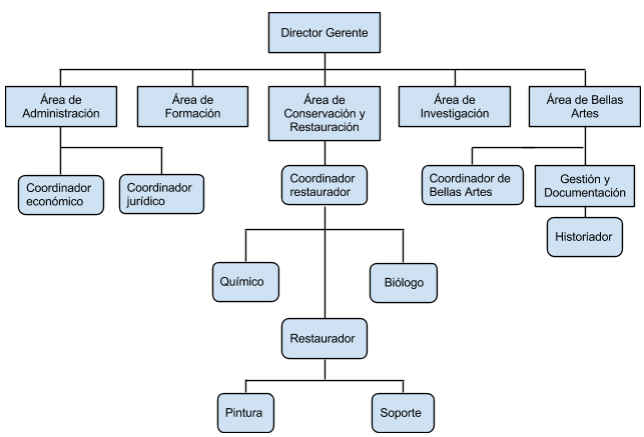
\includegraphics[width=350px]{organigrama.png} \\
			\end{center}
			\newpage
			\begin{landscape}
			\subsubsection{Formulario OM-3}
			\begin{center}
				\begin{tabular}{| l | p{4cm} | p{2.8cm} | p{2cm} | p{2cm} | p{3cm} |
				p{2.2cm} |}
					\hline
					\textbf{Nº} & \textbf{Tarea} & \textbf{Realizada por} & \textbf{¿Donde?} & \textbf{Recursos de conocimiento} &
					\textbf{¿Intensivo en conocimiento?} & \textbf{Importancia}\\
					\hline
					1 & Negociación del cuadro (valoración) & Director gerente & Despacho del
					director & Si & Si & Si\\
					\hline
					2 & Gestión de clientes & Área de administración & Área de administración
					& Si & No & Si\\
					\hline
					3 & Manipulación de personal & Área de administración & Área de
					administración & No & No & Si\\
					\hline
					4 & Información histórica del cuadro & Área de bellas artes & Área de
					bellas artes & Si & No & Si\\
					\hline
				\end{tabular}
			\end{center}
			\end{landscape}
			\newpage
			\begin{landscape}
			\begin{center}
				\begin{tabular}{| l | p{4cm} | p{2.8cm} | p{2cm} | p{2cm} | p{3cm} |
				p{2.2cm} |}
					\hline
					\textbf{Nº} & \textbf{Tarea} & \textbf{Realizada por} & \textbf{¿Donde?} & \textbf{Recursos de conocimiento} &
					\textbf{¿Intensivo en conocimiento?} & \textbf{Importancia}\\
					\hline
					5 & Prediagnóstico del cuadro & Área de conservación & Deslocalizado & Si
					& Si & Si\\
					\hline
					6 & Diagnóstico del cuadro & Área de conservación y restauración & Taller &
					Si & Si & Si\\
					\hline
					7 & Reparacion del cuadro & Área de conservación y restauración & Taller &
					Si & Si & Si\\
					\hline
					8 & Elaboración de presupuesto & Área de administración & Área de
					administración & No & No & No\\
					\hline
				\end{tabular}
			\end{center}
			\end{landscape}
			\newpage
			\begin{landscape}
			\subsubsection{Formulario OM-4}
			\begin{center}
				\begin{tabular}{| p{5cm} | p{2.4cm} | p{2cm} | p{2cm} | p{2cm} | p{2cm} |
				p{2cm} |}
					\hline
					\textbf{Recurso de conocimiento} & \textbf{Pertenece a} & \textbf{Usado en} & \textbf{¿Forma correcta?} & \textbf{¿Lugar correcto?} &
					\textbf{¿Tiempo correcto?} & \textbf{¿Calidad concreta?}\\
					\hline
Negociación del cuadro
& Director gerente
& 5,6,7,8
& Si
& Si
& No, a veces se tarda demasiado. 
& Si.\\
					\hline
Prediagnóstico 
& Area de conservacion
& 6,7,8
& Si
& No, a veces se hace fuera del taller.
& No, a veces se tarda demasiado. 
& Si\\
					\hline
Diagnóstico
& Área de conservación
& 7,8
& Si
& Si
& No, se tarda demasiado.
& Si\\
					\hline
Restauración del cuadro
& Área de conservación
& 
& Si
& Si
& Si
& Si\\
					\hline
				\end{tabular}
			\end{center}
			\end{landscape}
			\newpage
			\subsubsection{Formulario OM-5}
			\begin{center}
				\begin{tabular}{| p{4.5cm} | p{7cm} |}
					\hline
					\textbf{Viabilidad empresarial} & 
					\textbf{1. ¿Cuáles son los beneficios para la organización con la adopción
					de la solución?}\\
					& La empresa podrá acceder a nuevos proyectos ya que el
					SBC agilizará el proceso de diagnóstico.\\
					& \\
					& \textbf{2. ¿Cómo es el valor añadido esperado?}\\
					& Se espera que gracias al SBC se podrá realizar todos los proyectos que
					hasta ahora no han podido ser aceptados. Gracias a esto ConservArt podrá acceder a proyectos internacionales.\\
					& \\
					& \textbf{3. ¿Se requieren cambios organizacionales?}\\
					& No\\
					\hline
					\textbf{Viabilidad técnica} & 
					\textbf{1. ¿Existen aspectos críticos relativos al tiempo, calidad,
					recursos necesarios, etc?}\\
					& Si, el tiempo que se dedicaba para el diagnóstico era demasiado alto.
					Gracias al SBC estos tiempos disminuyen mucho.\\
					& \\
					& \textbf{2. ¿Cómo es de compleja la interacción con el usuario?}\\
					& La interacción con el usuario no es nada compleja. La aplicación es
					bastante intuitiva.\\
					& \\
					& \textbf{3. ¿Qué complejidad tiene la solución propuesta desde el punto de
					vista del conocimiento y los procesos de razonamiento desarrollado?}\\
					& La solución propuesta presenta la tarea de diagnóstico.
					Ésta viene detallada en la librería de CommonKads.\\
					\hline
				\end{tabular}
			\end{center}
			\newpage
			\begin{center}
				\begin{tabular}{| p{4.5cm} | p{7cm} |}
					\hline
					\textbf{Viabilidad del proyecto} & 
					\textbf{1. ¿Existe el compromiso por parte de ConservArt para llevar a
					cabo el proyecto?}\\
					& Si, la empresa se implica por completo.\\
					& \\
					& \textbf{2. ¿Está disponible el conocimiento y las capacidades
					requeridas?}\\
					& Si, están disponibles.\\
					& \\
					& \textbf{3. ¿Son realistas las expectativas relacionadas con el proyecto
					y los resultados?}\\
					& Si, ConservArt es una empresa en expansión y muchos clientes están
					esperando sus servicios.\\
					\hline
					\textbf{Acciones propuestas} & 
					\textbf{1. ¿Cuáles son los resultados, costes y beneficios esperados?}\\
					& El coste del sistema basado en conocimiento es alto en sus inicios. A la
					larga, sin embargo, permitirá a la empresa abordar proyectos en todo el
					mundo.\\
					& \\
					& \textbf{2. ¿Qué acciones se deben tomar dentro del proyecto para alcanzar
					dicha solución?}\\
					& ConservArt debe implicarse por completo con la realización del Sistema
					Basado en Conocimiento si quiere que el desarrollo de este tenga el éxito deseado.\\
					& \\
					& \textbf{3. Si las circunstancias que rodean a la organización cambian
					(tanto externas como internas), ¿bajo qué condiciones es apropiado
					reconsiderar las decisiones tomadas?}\\
					& La creación del Sistema Basado en Conocimiento afecta sólo a tareas agrupadas en dos departamentos. estos departamentos son pilares de la organización así que siempre deben formar parte de ella. Eso hace que la aplicación no se vea afectada por ninguna de estas causas.\\
					\hline
				\end{tabular}
			\end{center}
		\newpage
		\subsection{Modelo de tareas}
			\subsubsection{Formulario TM-1}
			Hay que hacer uno por cada tarea
			\begin{center}
				\begin{tabular}{| l | l |}
					\hline
					\textbf{Tarea} & \\
					\hline
					\textbf{Organización} & \\
					\hline
					\textbf{Objetivo y valor} & \\
					\hline
					\textbf{Dependencias y flujos} & \\
					\hline
					\textbf{Objetos manipulados} & \\
					\hline
					\textbf{Tiempo y control} & \\
					\hline
					\textbf{Agentes} & \\
					\hline
					\textbf{Conocimiento y capacidad} & \\
					\hline
					\textbf{Recursos} & \\
					\hline
					\textbf{Calidad y eficiencia} & \\
					\hline
				\end{tabular}
			\end{center}
			\subsubsection{Formulario TM-2}
			Hay que hacer uno por cada elemento de conocimiento usado en una tarea
			\begin{center}
				\begin{tabular}{| l | l |}
					\hline
					\textbf{Nombre} & \\
					\hline
					\textbf{Poseído por} & \\
					\hline
					\textbf{Usado en} & \\
					\hline
					\textbf{Dominio} & \\
					\hline
				\end{tabular}
				\\
				\textbf{}
				\\
				\begin{tabular}{| p{6.3cm} | l | p{3.8cm} |}
					\hline
					\textbf{Naturaleza del conocimiento} & \textbf{(si/no)} & \textbf{¿Cuello
					de botella?}\\
					\hline
					\textbf{Forma, riguroso} & & \\
					\hline
					\textbf{Empírico, cuantitativo} & & \\
					\hline
					\textbf{Específico del dominio} & & \\
					\hline
					\textbf{Basado en la experiencia} & & \\
					\hline
					\textbf{Basado en la acción} & & \\
					\hline
					\textbf{Incompleto} & & \\
					\hline
					\textbf{Incierto, puede ser incorrecto} & & \\
					\hline
					\textbf{Cambia con rapidez} & & \\
					\hline
					\textbf{Difícil de verificar} & & \\
					\hline
					\textbf{Tácito, difícil de transferir} & & \\
					\hline
					\textbf{Forma de conocimiento} & \textbf{(si/no)} & \textbf{¿Cuello
					de botella?}\\
					\hline
					\textbf{Mental} & & \\
					\hline
					\textbf{Papel} & & \\
					\hline
					\textbf{Electrónica} & & \\
					\hline
					\textbf{Habilidades} & & \\
					\hline
					\textbf{Otros} & & \\
					\hline
					\textbf{Disponibilidad del conocimiento} & \textbf{(si/no)} & \textbf{¿Cuello
					de botella?}\\
					\hline
					\textbf{Limitaciones en tiempo} & & \\
					\hline
					\textbf{Limitaciones en espacio} & & \\
					\hline
					\textbf{Limitaciones en acceso} & & \\
					\hline
					\textbf{Limitaciones en calidad} & & \\
					\hline
					\textbf{Limitaciones en forma} & & \\
					\hline
				\end{tabular}
			\end{center}
		\subsection{Modelo de agentes}
			\subsubsection{Formulario AM-1}
			Hay que crear uno por cada agente
			\begin{center}
				\begin{tabular}{| l | l |}
					\hline
					\textbf{Nombre} & \\
					\hline
					\textbf{Organización} & \\
					\hline
					\textbf{Implicado en} & \\
					\hline
					\textbf{Se comunica con} & \\
					\hline
					\textbf{Conocimiento} & \\
					\hline
					\textbf{Otras competencias} & \\
					\hline
					\textbf{Responsabilidad y restricciones} & \\
					\hline
				\end{tabular}
			\end{center}
		\subsection{Formulario resumen}
			\subsubsection{Formulario OTA-1}
			\begin{center}
				\begin{tabular}{| l | l |}
					\hline
					\textbf{Impactos y cambios en la organización} & \\
					\hline
					\textbf{Impactos y cambios en tareas y agentes} & \\
					\hline
					\textbf{Actitudes y compromisos} & \\
					\hline
					\textbf{Acciones propuestas} & \\
					\hline
				\end{tabular}
			\end{center}
	\newpage
	\section{Modelado conceptual}
		\subsection{Modelo de conocimiento}
			\subsubsection{Formulario KM-1}
			
		\newpage
		\subsection{Modelo de comunicación}
			\subsubsection{Formulario CM-1}
			Hay que hacer uno por cada transacción, quizás
			\begin{center}
				\begin{tabular}{| l | l |}
					\hline
					\textbf{Nombre de transacción} & \\
					\hline
					\textbf{Objetos de información} & \\
					\hline
					\textbf{Agentes involucrados} & \\
					\hline
					\textbf{Plan de comunicaciones} & \\
					\hline
					\textbf{Restricciones} & \\
					\hline
					\textbf{Especificaciones del intercambio de información} & \\
					\hline
				\end{tabular}
			\end{center}
			\subsubsection{Formulario CM-2}
			Hay que hacer uno por cada transacción, quizás
			\begin{center}
				\begin{tabular}{| l | l |}
					\hline
					\textbf{Transacción} & \\
					\hline
					\textbf{Agentes involucrados} & \\
					\hline
					\textbf{Ítems de información} & \\
					\hline
					\textbf{Especificaciones de los mensajes} & \\
					\hline
					\textbf{Control sobre mensajes} & \\
					\hline
				\end{tabular}
			\end{center}
	\newpage
	\section{Modelado de diseño}
		\subsection{Modelo de diseño}
			\subsubsection{Formulario DM-1}
			\begin{center}
				\begin{tabular}{| l | l |}
					\hline
					\textbf{Decisiones arquitectónicas} & \textbf{Formato} \\
					\hline
					\textbf{Organización de los subsistemas} & \\
					\hline
					\textbf{Modelo de control} & \\
					\hline
					\textbf{Descomposición de subsistemas} & \\
					\hline
				\end{tabular}
			\end{center}
			\newpage
			\subsubsection{Formulario DM-2}
			\begin{center}
				\begin{tabular}{| p{4.8cm} | p{6.5cm} |}
					\hline
					\textbf{Producto software} & SDJS - RCPTTE \\
					\hline
					\textbf{Hardware potencial} & El sistema se va a instalar en un servidor
					web. Es una aplicación sencilla donde el cálculo se realiza en el cliente por lo que el servidor se limita a servir peticiones.\\
					\hline
					\textbf{Hardware de desarrollo} & Para el desarrollo del sistema contamos
					con equipos normales y portátiles de una potencia y costes moderados.\\
					\hline
					\textbf{Librería de visualización} & Para la visualización de la aplicación
					se va a emplear una aplicación web realizada con HTML5, CSS3 y Javascript.\\
					\hline
					\textbf{Lenguaje de implementación} & El lenguaje empleado para el motor de
					inferencia es Javascript. Hemos encontrado un motor de inferencia realizado por Jose Manuel Ayala Wilson y licenciado bajo GNU GPL V3 que podemos reutilizar.\\
					\hline
					\textbf{Representación del conocimiento} & La representación del
					conocimiento se realizará en una base del conocimiento hecha en Javascript y formada por preguntas, respuestas, hechos y reglas.\\
					\hline
					\textbf{Protocolos de interacción} & La aplicación sólo es accesible
					mediante el navegador al ser una página web. Sin embargo tiene un formato que permite su acceso desde PC, Tablet o Smartphone.\\
					\hline
					\textbf{Control de flujo} & El flujo de la aplicación consistirá en el uso
					de un motor de inferencias y una serie de preguntas cuya respuesta almacenará hechos en una base del conocimiento. Eventualmente la aplicación alcanzará una conclusión.\\
					\hline
					\textbf{Soporte para CommonKADS} & Vamos a emplear Aptana Studio para el
					desarrollo de la aplicación web, Git para realizar el proyecto de forma colaborativa y el plugin TeXlipse para Aptana para el desarrollo de los modelos CommonKADS en Latex.\\
					\hline
				\end{tabular}
			\end{center}
			\subsubsection{Formulario DM-3}
			\begin{center}
				\begin{tabular}{| l | l |}
					\hline
					\textbf{Elemento de la arquitectura} & \textbf{Elementos típicos de
					decisión} \\
					\hline
					\textbf{Controlador} & \\
					\hline
					\textbf{Tarea} & \\
					\hline
					\textbf{Método de la tarea} & \\
					\hline
					\textbf{Inferencia} &  \\
					\hline
					\textbf{Método de la inferencia} & \\
					\hline
					\textbf{Rol estático} & \\
					\hline
					\textbf{Rol dinámico} & \\
					\hline
					\textbf{Base de conocimiento} & \\
					\hline
					\textbf{Vistas} & \\
					\hline
				\end{tabular}
			\end{center}
			\subsubsection{Formulario DM-4}
			\begin{center}
				\begin{tabular}{| l | l | l |}
					\hline
					\textbf{Elemento} & \textbf{Decisión de diseño} & \textbf{Comentarios} \\
					\hline
					\textbf{Controlador} &  & \\
					\hline
					\textbf{Método de la tarea} &  & \\
					\hline
					\textbf{Roles dinámicos} &  & \\
					\hline
					\textbf{Inferencias} &  & \\
					\hline
					\textbf{Métodos de las inferencias} &  & \\
					\hline
					\textbf{Bases de conocimiento} &  & \\
					\hline
					\textbf{Vistas de los objetos} &  & \\
					\hline
				\end{tabular}
			\end{center}
\end{document}